As a result of the investigation in chapter \ref{ch:methods}, a small use case scenario was conducted. In detail, the development process of an \emph{error detection service} was investigated by means of the development phases featured in section \ref{sec:service-development-process}. Due to the scarce reference material related to this topic, the use case scenario is rather short and quite theoretical. However, it provides a good example on what a service development process may look like.
\\
\\
At the end of the first four phases, which are concerned with the conceptual development, the service contract is issued. Subsequently follows the actual implementation of the service by a developer, who was (most likely) not included in the preceding design phases. Therefore, the contract must provide all the necessary information for the implementation process, leaving no ambiguities or open questions.

It is then up to the developer to decide how the service will be implemented, e.g. which programming language or approach to use. The outcome is a certain architecture, which can be based on any arbitrary technology. 



\section{Service Investigation/Planning}


\begin{description}
\item [Scope of the service].
The service should be capable of detecting an error within a given ECR and act accordingly. Therefore it needs the signal of all the sensors it should mirror, as well as clock signal for creating sampling times.
\item [Required capabilities].
	\begin{itemize}
	\item Detection an error in one of the sensors.
	\item Restart of an erroneous sensor.
	\item Purging the service from the service repository if more than two sensors fail and errors can no longer be detected.
	\end{itemize}
\item [Non-required capabilities].
	\begin{itemize}
	\item Detection of a fault.
	\item Detection of a failure.
	\end{itemize}
\end{description}



\section{Service Inventory Analysis}


The error detection service will require:
\begin{itemize}
\item A \emph{clock service} for creating sampling times,
\item A \emph{fault detection service} for detecting a fault in one of the mirrored services,
\item A \emph{management service for the service repository} to update the repository in case of an erroneous service, and additionally perhaps
\item A \emph{service for restarting another service}, which is erroneous.
\end{itemize}

During operation, it will also need the redundant service inside the ECR, whose functionality shall be checked for errors. Of course they should feature different implementations on independent hardware components, so that an error could not emerge in multiple services at the same time.


\section{Service Oriented Analysis}


Concerning the naming, the example service should be in accordance with the AUTOSAR naming conventions \cite{autosar_system_modelling}. Accordingly, a suitable candidate would be \textbf{error\_detection}.

The \emph{service normalisation} and \emph{service candidate review} are not really doable just theoretically. Therefore, it shall be assumed that the example service has no overlapping functionality and has passed the review.





\section{Service Oriented Design}

Unfortunately, the service contract templates, which are designed by Arrowhead, were not yet available at the time this thesis was written. Accordingly, there could be no example contract be established.


\section{Possible Implementation}

A possible architecture resulting from the service of this use case is a triple modular redundancy approach (cf. section \ref{sec:error-detection-service}), as depicted in figure \ref{fig:example-service-architecture}. 


\begin{figure}[ht]
\centering
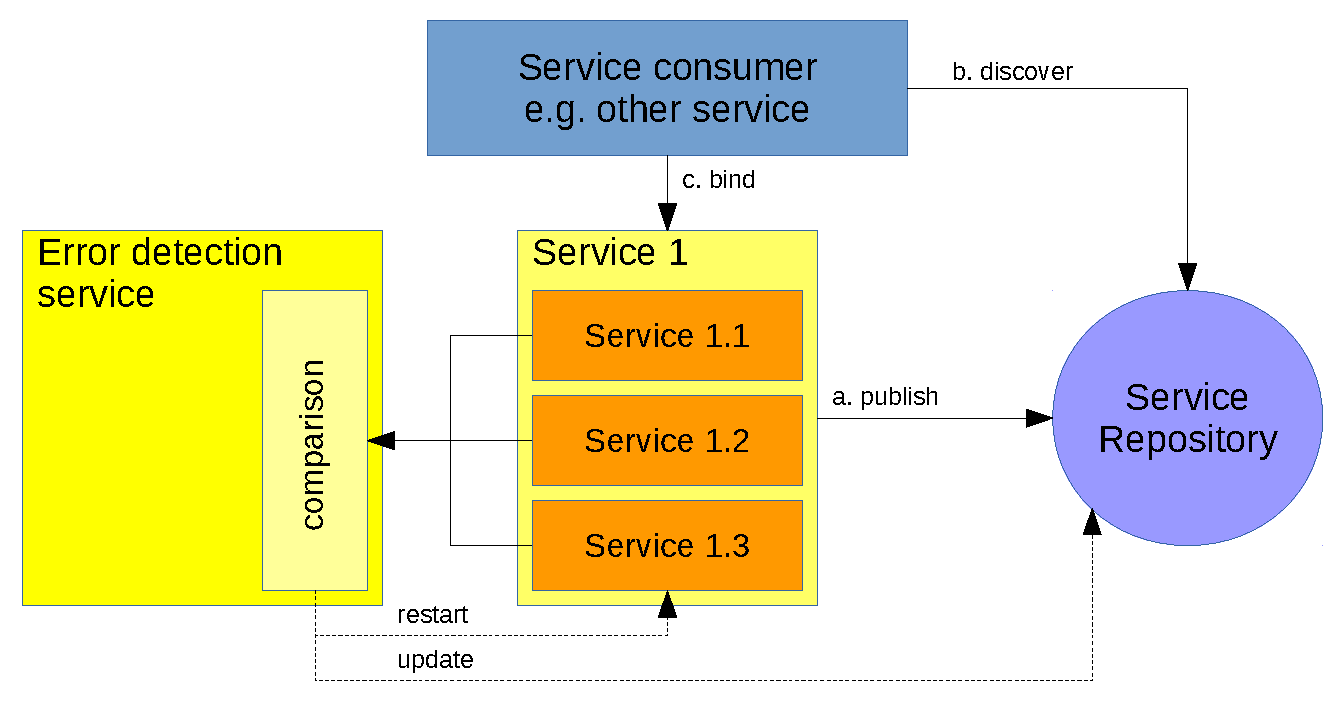
\includegraphics[width=\textwidth]{error-detection-service.pdf}
\caption{Possible architectural implementation of the example service.}
\label{fig:example-service-architecture}
\end{figure}